\chapter{Sequence probability modelling}

Generating a "Bach-like" piece of music can be understood as drawing a random
sample from a distribution over musical scores which is statistically similar
to Bach's own compositions. Thus, we interpret the problem as one of
\emph{categorical sequence modeling}.

This type of problem has been well studied. In speech recognition, language
models parameterizing distributions over sentences are used as priors to refine
transcriptions.

However, since our model has to be able to generate Bach, we must be able to
sample from it. This rules out a broad class of sequence models, including
back-off N-grams and other interpolated language models.

Fortunately, low order N-grams and standard HMM-based models are sampleable and
thus can be used as baselines.

\section{Feedforward neural networks}

Increasing context window size is not always a good solution:
\begin{itemize}
    \item Too small $\implies$ no long-term dependencies captured
    \item Not all $N$-grams observed $\implies$ need back-off and discounting
\end{itemize}

How do we handle variable length inputs?

\section{Recursive neural networks}

Carry memory $s_t$ through time $t$, ``summary of infinite context duration
i.e.\ all previously processed data''

Share weights $\matr{U}, \matr{V}, \matr{W}$ over $t$ since performing same
task at each time i.e.\ modeling $P(o_t | s_t, x_t) = \softmax(V s_t)$.

\begin{figure}[htpb]
    \centering
    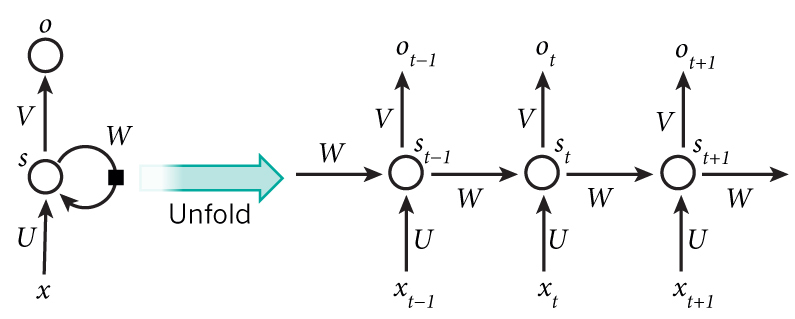
\includegraphics[width=0.8\linewidth]{Figures/rnn.jpg}
    \caption{\todo{Redraw in xy}}
\end{figure}

\begin{align}
    \s_t &= f(\U \x_t + \W \s_{t-1}) \\
    \o_t &= \softmax( \V \s_t)
\end{align}

$f$ is usually $\tanh$ or ReLU.

\begin{enumerate}
    \item Memory/state $\s_t$ summarizes ALL previous information
    \item $\U, \V, \W$ parameters are shared across all $t$. Reflects
        that the same task is being performed at each input i.e.\
        invariance over time. Reduces number of parameters.
\end{enumerate}


RNNs are a sequence model similar to HMMs in that they model the conditional
distribution of next frames given the previous context. However, RNNs additionally
pass along "hidden state" which summarizes contextual information from a potentially
infinite context window.

In practice, it is observed that the hidden state does not capture long range
dependencies well and tend to suffer from vanishing/exploding gradient during
training. LSTMs are an improved RNN architecture which solve both of these
problems by introducing gates on the inputs, hidden state, and outputs. GRUs are
a variation of LSTMs which ties the weights to the input and forget gates.

\begin{enumerate}
    \item Language modeling
        \begin{enumerate}
            \item Model $P(\m), \m \in V^T, T \in \NN$
            \item Train to predict the distribution of the next note in the
                melody i.e.\ $\o_t = P(\m_t | \m_{1:t-1})$
            \item $\m_{t-N:t-1}$ is given explicitly as input $\x_t$ and
                $\s_{t}$ captures information from before $t-N$
            \item See \cite{Martens2011}, \cite{Mikolov2011}, \cite{Mikolov2010}
        \end{enumerate}
    \item Machine translation
        \begin{enumerate}
            \item~\\
                \begin{figure}[htpb]
                    \centering
                    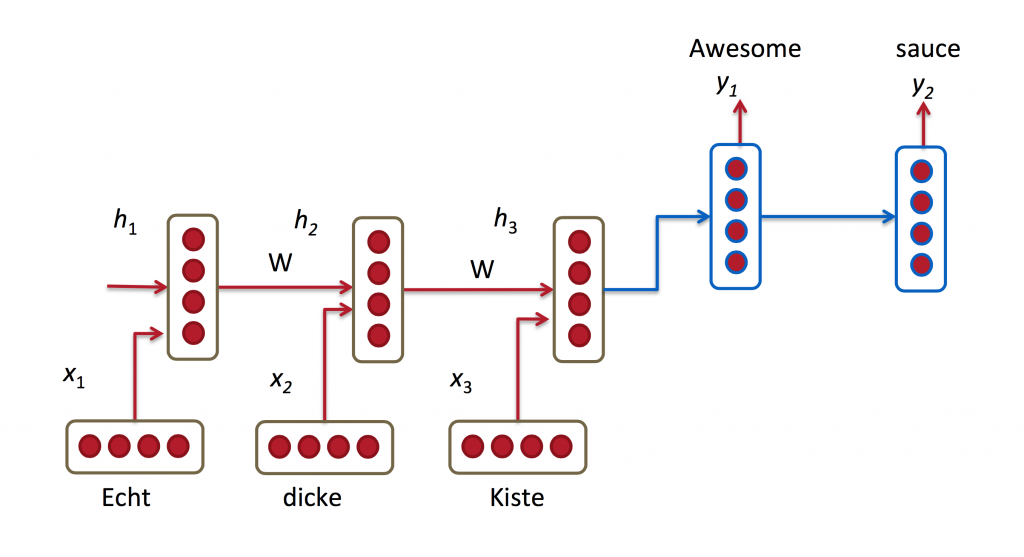
\includegraphics[width=0.8\linewidth]{Figures/rnn-mt.png}
                    \caption{\todo{Redraw in xy}}
                \end{figure}
            \item Input is a sequence of words in source language $\leftrightarrow$
                sequence of notes in $V$
            \item Output is four sequences of notes, one for each of the 4 chorale parts.
            \item Architecture difference: output only starts after input is completely
                consumed because first word of translated sentence may require information
                from complete sentence input
                \begin{enumerate}
                    \item This could be mitigated with bidirectional LSTMs \cite{Graves2005}
                    \item Could also try Neural MT \cite{Bahdanau2015}, whose attention
                        neural network could be used to extract insights about which parts
                        of the overall melody influences decision making within local regions
                        of music
                \end{enumerate}
            \item See \cite{Liu2014}, \cite{Auli2013}, \cite{Sutskever2014}.
        \end{enumerate}
\end{enumerate}

